\section{Validation and grid design ComFLOW}
\label{ch: validation comflow}
In this thesis, a breakwater is designed to provide shelter to a floating island from incoming waves. To arrive at the best design, the hydrodynamic behaviour of different geometries must be analysed, to assess which design offers the best performance. To simulate multiple variations of the geometry, a \acrshort{cfd} software method is used: ComFLOW. This method numerically solves the Navier-Stokes equations, and thereto, the computational domain is covered by a fixed Cartesian grid. A coarser grid generally means faster simulations, so a coarse grid is desired to save computational power and maximise the total number of simulations performed in a limited amount of time.  On the other hand, the grid must be fine enough to give reliable results that converge to a static value. In other words,  the result of the final grid must be the same as when the grid is refined further. And the comparison must be made with reality, to quantify the deviation from the ComFLOW result, to be able to draw conclusions from the simulations.\\
\\

Also, ComFLOW comes with a lot of different settings. The effects of different settings and different grids were extensively analysed during the first months of this graduation thesis. This resulted in certain settings and grid characteristics that gave the best performance, which are presented in the following sections. So, only the most important and useful results of this extensive analysis are discussed. The ComFLOW settings used are introduced in Section \ref{sec: possible settings ComFLOW}, and the outline of the grid is explained in \ref{sec: general outline grid}. Different refinements of this outline are analysed in sections \ref{sec: prop of free surface waves} and \ref{sec: box-type breakwater}. Where \ref{sec: prop of free surface waves} studies the propagation of free surface waves through the domain without interference with a geometry, to quantify the numerical dissipation and reflection at the boundaries and refinement edges. And \ref{sec: box-type breakwater} compares the results of ComFLOW when regular waves interfere with a box-type breakwater with linear wave theory. Finally, the dissipation of wave energy through wave breaking in ComFLOW is tested by comparing its results with an experiment in which waves plunged over a breaker bar in Section \ref{sec: Dissipation}, performed by \citet{breakerbarexperiment}.


% -grid generation: realistic results, but most efficient in terms of computation time/expensiveness\\
% -checked by three different methods, first the settings are chosen in which less numerical dissipation as possible is achieved, to check the average wave height over the complete length of the domain. (in first paragraph)\\
% -reflection is validated by the Macagno formula and the forces experienced (second paragraph).\\
% -An experiment with a breaker bar is mimicked to validate the model on dissipation


\section{Settings ComFLOW}
\label{sec: possible settings ComFLOW}
ComFLOW can be used with lots of different settings, integration and convection schemes, wave models, etc. Various wave settings that are applicable to this thesis are studied and discussed in this section. Most of the information comes from the ComFLOW reference page \citep{poseidon_comflow_reference_page}. Also, the final settings used that gave the best performance are given in this section.

\subsection{Integration method}

Two different integration methods can be used: Forward-Euler and Adams-Bashforth. Forward Euler is a single-step method which refers to only one previous point and its derivative to determine the current value. Adams-Bashforth is a two-step explicit method. The influence of both methods on the simulation results and computation time was found to be negligible.\\
\\
\textbf{Adams-Bashfort was chosen for future simulations.}

\subsection{Boundary conditions}
At the boundaries of the domain, the inflow and outflow conditions can be specified. The various types are
\begin{itemize}
    \item Basic inflow condition: Imposes incoming flow by means of a Dirichlet condition for the velocity and the water level. 
    \item \acrfull{gabc}: An extension of the Sommerfield boundary condition (using a wave velocity, which is calculated from the wave period and wave number) with an approximation of the linear dispersion relation in terms of $k h$, in combination with vertical derivatives of the solution variables \citep{Wellens2020}. 
    \item Pressure Neumann: The Neumann boundary condition is obtained by applying the normal component of the momentum equation at the boundary \citep{Abdallah1988} 
    
    % Pressure and water height in the exterior of the domain are approximated using constant extrapolation. This is a very simple boundary condition and does not perform very well in wave simulations.
    \item Pressure Dirichlet: The Dirichlet boundary condition is obtained by integrating the tangential component of the momentum equations along the boundary \citep{Abdallah1988}.
    \item Free slip: At free-slip boundaries, the tangential velocities in the exterior are set equal to those in the interior such that the viscous stresses become zero. The liquid distribution is assumed to be uniform across the boundary. 
\end{itemize}


\textbf{The \acrshort{gabc} was found to be the best performing in terms of stability and reflection and is used for future simulations.}

\subsection{Numerical settings}
\label{subsec: numercial settings validation}
\subsubsection{Linear solver}

The linear solver is used for solving the pressure Poisson equations, and when quasi-implicit discretization is used for diffusion, the solver is also used for solving the intermediate solution of the momentum equations. The different options are as follows:
\begin{itemize}
    \item \textbf{BiCGSTAB + ILU} preconditioner with special drop tolerance. 
    \item \textbf{SOR} with improved search algorithm. 
\end{itemize}
Only the first of the listed solvers (\textbf{BiCGSTAB + ILU}) is compatible with all ComFLOW simulation settings. The preconditioner in this solver takes care of the special matrix structure near the GABC boundaries and is able to cope with large density variations in two-phase flow simulations.\\
For most one-phase simulations, the solver \textbf{SOR} provides a satisfactory alternative. The \textbf{SOR} solver cannot be used for two-phase simulations or simulations that include a GABC boundary condition.\\
There are more options, but they do not support local grid refinement and have not been parallelised. 

\textbf{The first mentioned: BiCGSTAB + ILU will be used for future simulations}

\subsubsection{Stopping criterion}
The number of solver iterations is determined by two mechanisms. First, the number of iterations is bounded by the setting: 'iter\_max'. This value should be chosen large enough to allow the solver to reach the desired precision and small enough to minimise computational demand.  Second, the solver iterations are controlled by the residual tolerance. In general, smaller values result in more iterations, but improve the accuracy of the solution. The convergence behaviour (error w.r.t. iteration count) depends on the chosen solver. A value of "1.0E-6" is generally a good value, but a useful value in the case of \textbf{wave simulations is "1E-8", so this value will be used for future simulations.}


\subsubsection{Convection scheme}
ComFLOW supports two categories of discretization schemes for convection:
\begin{itemize}
    \item First-order upwind
    \item Second-order central
\end{itemize}
These schemes handle the discretization of convective terms in finite-volume equations. To illustrate both methods, consider the following one-dimensional linear advection term.
\begin{equation}
\frac{\partial u}{\partial t}+a \frac{\partial u}{\partial x}=0
\label{eq: discretization wave}
\end{equation}
It describes a wave propagating in the x-direction with velocity \textit{a}. This can be discretised as
\begin{equation}
\begin{array}{ll}
\frac{u_{i}^{n+1}-u_{i}^{n}}{\Delta t}+a \frac{u_{i}^{n}-u_{i-1}^{n}}{\Delta x}=0 & \text { for } \quad a>0 \\
\\
\frac{u_{i}^{n+1}-u_{i}^{n}}{\Delta t}+a \frac{u_{i+1}^{n}-u_{i}^{n}}{\Delta x}=0 & \text { for } \quad a<0
\end{array}
\end{equation}
where \textit{n} refers to the dimension in time t and \textit{i} refers to the dimension in space x. So, cell \textit{i-1} is the cell left to cell \textit{i} and \textit{i+1} right of \textit{i}. If \textit{a} is positive, the travelling wave solution of the above equation propagates towards the right, the left side of \textit{i} is called the \textit{upwind} side and the right side is the \textit{downwind} side. When \textit{a} is negative, it is the other way around.\\
\\
The second-order central discretization of equation \ref{eq: discretization wave} looks like
\begin{equation}
    \frac{ u_{i}^{n+1}-u_{i}^{n}}{\Delta t}+a \frac{u_{i+1}^{n}- 2u_{i}^{n} + u_{i-1}^{n}}{\Delta x}=0 
\end{equation}
What is good to note, is that the second-order central method uses three cell points in each discretisation, while the first-order upwind method uses two cells. \textbf{The first-order upwind scheme tends to be more stable and gives better dissipation characteristics, so will be for future simulations.} This is elaborated more in \ref{subsec: breakerbar on convection scheme} 


\subsection{Wave model}
An important application of the ComFLOW programme is the simulation of wave impact on offshore structures. ComFLOW provides various built-in wave models, as well as the possibility to import custom data by means of plug-ins. By means of plug-ins and coupling to other software, it is possible to simulate a wide range of other wave conditions (e.g. irregular waves). Wave models can be used for initialisation or as input for boundary conditions.
\subsubsection{Airy wave theory}
The Airy wave model defines the wave elevation by a cosine:
\begin{equation}
    \eta(x,t) = A\cos(\omega t - kx + \epsilon) 
\end{equation}
where $A$ is the amplitude $\omega$ the frequency, $k$ the wave number, and $\epsilon$ the phase.

\subsubsection{Stokes wave theory}
ComFLOW provides second-order and fifth-order Stokes wave models, which are a nonlinear and periodic surface wave.

\subsubsection{Rienecker-Fenton wave theory}
Rienecker-Fenton wave theory gives more accurate wave kinematics than the 5th-order Stokes, especially in shallow water and for very steep waves.\textbf{This will be input for future simulations.}



\subsection{CFL number}
The CFL number automatically controls the time step in order to satisfy numerical stability restrictions without using unnecessary small time steps. It requires that the time step satisfies (at least) the following condition:


\begin{equation}
    CFL = \frac{ \Delta t |\mathbf{u}|}{\Delta x} \leq 1
\end{equation}
where $\Delta t$ is the time step size, $\Delta x$ is the local grid spacing, and $u$ is the magnitude of the local fluid velocity. In other words, this condition states that the fluid must not propagate more than one grid cell per time step. \\
\\
The above is called $CFL_{default}$. There is another CFL condition that can and should be applied when simulating waves: the $CFL_{wave}$ condition. This condition does the same thing as the equation above, but with the wave propagation velocity. This means that waves do not propagate more than one cell length per time step. For nonbreaking waves, the propagation speed of a wave is typically higher than the orbital velocity. When this is the case $CFL_{wave}$ would be the limiting factor in determining the time step.\\
\\
\textbf{The following CFL numbers will be used in the future simulations:}
\begin{itemize}
    \item $CFL_{default, min}$ = 0.2
    \item $CFL_{default, max}$ = 0.85
    \item $CFL_{wave, min}$ = 0.5
    \item $CFL_{wave, max}$ = 0.5
\end{itemize}

A wide range between $CFL_{default, min}$ and $CFL_{default, max}$ is chosen to allow the programme to easily change between different time steps without exceeding the $CFL_{default}$ range.


\section{General outline grid}
\label{sec: general outline grid}



In the past months, a lot of different settings and grid refinements were tested. Initially, to make the simulation stable, extensive analyses have been done on its performance. This eventually led to the general outline of the grid, which is going to be used in future simulations. This general outline can be seen in Figure \ref{fig:complete grid}. Figure \ref{fig:zoomed grid} shows the same grid but zoomed in to see how the different refinements are arranged, which is also explained in further detail. The validation grid is 1056 m long (x=-270 m to 786 m) and 40 m high (z = -23 m to z = 17 m). At z = 0 is the waterline, and waves will enter the domain on the left and propagate toward the structure. The structure will have its wave-ward side between x = 50m and 140m (depending  on the structure's width) and the lee-side is always at x = 150m (this is kept constant because from a practical point of view; the transmitted wave height is analysed behind the structure). There are four different refinement levels present in the grid, which are enumerated from fine to coarse.
\begin{enumerate}
    \item The finest grid can be separated into three different areas. Just above and below the waterline and around the structure, a fine grid is present because high fluid velocities are expected here. And at the first 10 metres of the domain in the x-direction, next to the left boundary of the domain, this fine grid is required to allow the wave-generating boundary condition (\acrshort{gabc}) to perform optimally. In addition, the force on the structure is calculated by integrating the pressure over its boundary. This integration is done with the finite elements around the body: the number of cells. More elements produce a more accurate result and therefore a fine grid is required in order to give accurate results of the forces acting on the breakwater.
    \item The second finest grid is placed around the finest grid to ensure a smooth transition between the different refinement levels.
    \item The third refinement level covers the rest of the domain (with the exception of the area near the bottom). This part of the domain serves as a dissipation area. So, it is there to ensure that the wave energy that is reflected at the right boundary interferes as little as possible with the evaluation of the waves in refinement level 1. 
    \item Near the bottom, low fluid velocities are expected, which results in less numerical dissipation. So, here the coarsest grid is present to save computational power. This part does not reach the end of the domain, because different grid refinements are also not desired at the outer boundary.
\end{enumerate}


%  Around the waterline (from z = -5m until z = 9m) the grid is refined from the beginning of the domain: x - 270m, until x = 350m. This is done to have the least amount of numerical dissipation around the structure. Between x = -270m and x = -260m the same refinement is applied over the entire height of the grid, because the wave-generating boundary condition on the left-hand side of the domain does not perform optimally when different refinements are present over the z-axis. Some reflection occurs when a grid shifts in coarseness in the direction of wave propagation, especially from coarse to fine. Therefore, the same degree of refinement is chosen for the latter area as around the waterline. Around the geometry (edges of geometry plus 10 m) is also refined, with the same level of refinement as around the waterline, because at this position high speeds occur due to the presence of the geometry. At the bottom, a coarse grid was chosen in order to save computing power in the simulations. This is possible because of the low orbital velocity of the fluid near the bottom. The geometry ends at x = 150 m and all measurements are made between x = 150 m and x = 350 m, so at first sight the rest of the  (x>350m) is of no use. However, the right-hand boundary does not absorb 100\% of the wave energy, so the large space between x = 350 m and x = 786 m is needed so that the reflected wave energy at the boundary does not interfere with the simulation during execution. This is for the obvious reason that it takes some time for the wave to travel 872 m (from x=350 m to x=786m and back), but also because in this part of the domain there will be a relatively large amount of numerical dissipation (due to its coarseness) and thus not much wave energy is left when it has travelled all the way back into the refined domain

\begin{figure}[H]
    \centering
    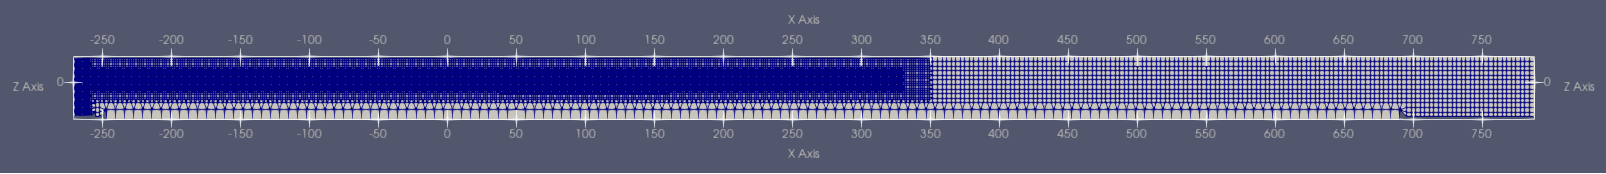
\includegraphics[width=\linewidth]{figures/Validation/grid_naked.png}
    \caption{Complete grid}
    \label{fig:complete grid}
\end{figure}
\begin{figure}[H]
    \centering
    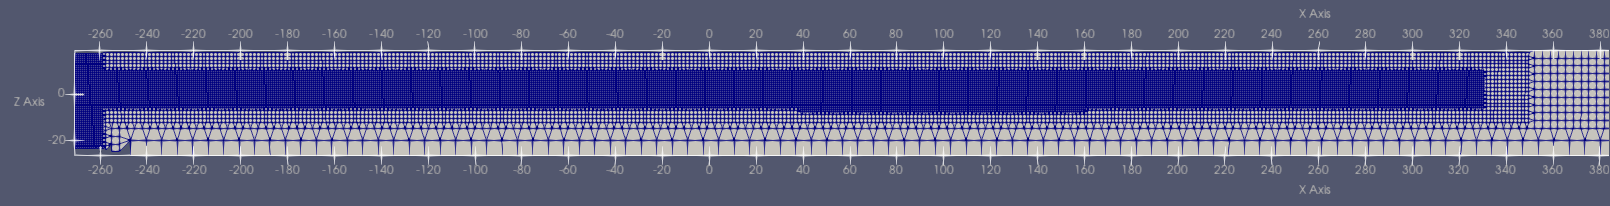
\includegraphics[width=\linewidth]{figures/Validation/grid_zoomed.png}
    \caption{Grid, zoomed on refinement}
    \label{fig:zoomed grid}
\end{figure}


Within this general outline, different refinements have been tested to obtain the optimal refinement. The different grid refinements are numbered from one to five and their characteristics are shown in Table \ref{tab:celldimensions}. The \textit{computation time} is the execution time of ComFLOW of one simulation of 250 seconds.

% Please add the following required packages to your document preamble:
% \usepackage{booktabs}
\begin{table}[H]
\centering
    \begin{tabular}{@{}ccccc@{}}
    \toprule
    grid number & finest cell width {[}mm{]} & finest cell height {[}mm{]} & number of cells & computation time \\ \midrule
    1           & 125                 & 125                  & 5.429.720 & 4 days \\
    2           & 250                 & 250                  & 1.486.840 & 13 hours \\
    3           & 500                 & 500                  & 442.420 & 2 hours \\
    4           & 825                 & 830                  & 209.600 & 1 hour \\ 
    5           & 1250                 & 1250                & 113.440 & 15 minutes  \\ \bottomrule
    \end{tabular}
    \caption{Grid properties}
    \label{tab:celldimensions}
\end{table}



% \subsection{orthogonality}
% \subsection{skewwness}

\section{Propagation of free surface waves}
\label{sec: prop of free surface waves}
%wave only
%Numerical dissipation \& reflection at boundary
%dissipation means high frequency components get smoothed out. Lower frequency oscillations damp at a much slower rate! 
%numerical dissipation iss not suposed to be in the behaviour of the original equations, but is introduced by using numerical approximations. 
%since first-order approximations cut off higher order terms, numerical dissipation occcurs when the higher harmonics are present, higher harmonics tend to have large excitations with small perturbations (since they scale with at least the x^2), so when time step or dimensional step gets large numerical dissipation will be large


The propagation of free surface waves is studied by simulating waves in grids alone, without the interference of any geometry. \textbf{For all simulations, including those in the following sections, 250 seconds of a regular wave was generated with the following characteristics: H = 0.5 m and T = 10.4 s}. The choice for such a long and shallow wave has been made to minimise the nonlinear terms present, in order to allow comparison with linear wave theories, which is elaborated more in Section \ref{sec: box-type breakwater}.\\
\\
Figure \ref{fig:averagewaveheight} shows the average wave height over the refined domain (-270m < x < 350m).  How this is determined is as follows; from each position in the domain, the average wave height is taken from the moment the waves are fully developed in the entire refined domain. Therefore, the time signal on the right side of the refined part of the domain (x = 350 m) is taken (see Figure \ref{fig:waterelevation350m}), from which it can be concluded that the first 125 seconds of simulation is the ramp up time. So, for every position along the x-direction of the domain the first 125 seconds of simulation is discarded, and a mean value of the wave height is determined. This is plotted over the entire length of the refined domain and results in Figure \ref{fig:averagewaveheight}. To see the percentage in which the average wave height varies over the domain, the y-axis of the graph is normalised with the height of the incoming wave.  


\begin{figure}[H]
     \centering
     \begin{subfigure}[b]{0.49\textwidth}
         \centering
         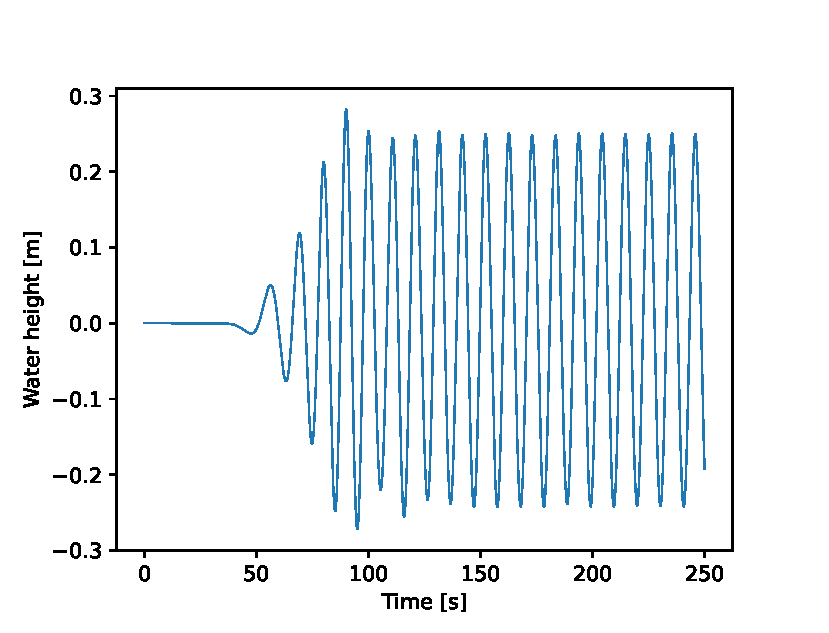
\includegraphics[width=\textwidth]{figures/Validation/water_elevation_350m_eps.eps}
        \caption{Water elevation at x = 350 m}
        \label{fig:waterelevation350m}
     \end{subfigure}
     \hfill
     \begin{subfigure}[b]{0.49\textwidth}
         \centering
        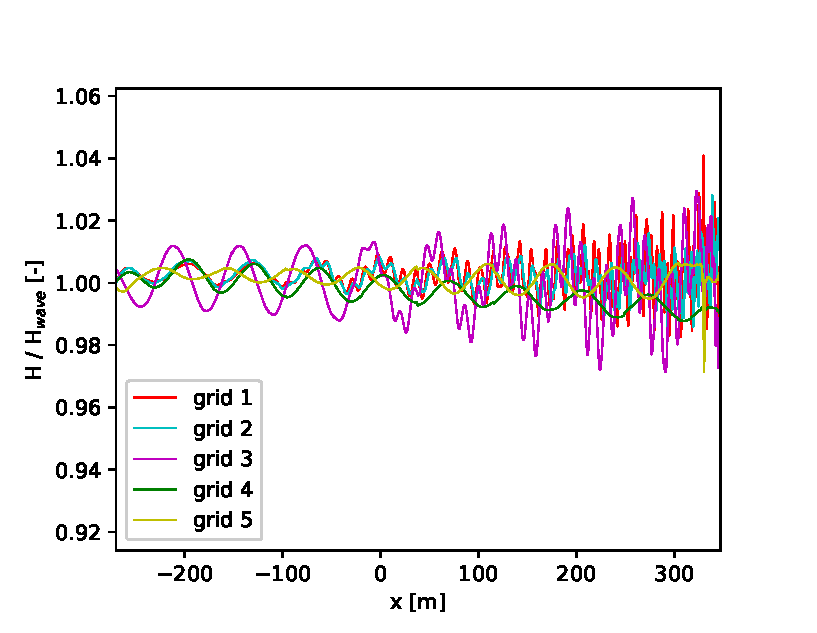
\includegraphics[width = \linewidth]{figures/Validation/numerical_dissipation_eps.eps}
        \caption{Average wave height over length grid}
        \label{fig:averagewaveheight}
     \end{subfigure}
     \caption{Water elevation over time and average wave height over the grid}
\end{figure}


% \begin{figure}
%     \centering
%     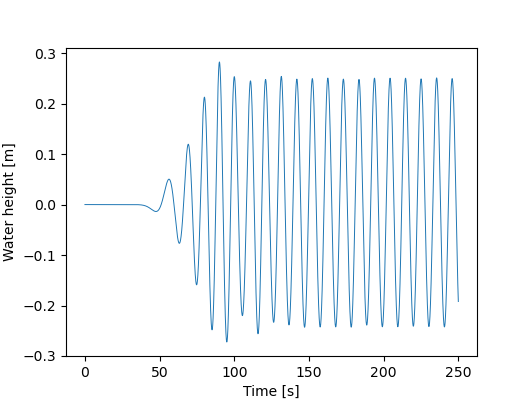
\includegraphics[width=\linewidth]{figures/Validation/water_elevation_350m.png}
%     \caption{Water elevation at x = 350 m}
%     \label{fig:waterelevation350m}
% \end{figure}


% % -general outline is determined by studying the numerical dissipation. And eventual result is: PICTURE OF OUTLINE OF GRID, WITH DIFFERENT REGIONS AND EXPLAIN THE REGIONS
% % -average wave height determination calculation\\
% % -- not going to show 100.000 plots of all the simulations, but to give an insight in the progression, the numerical dissipation first looked like this (few or one example)
% % -- eventually, looked like this: with grid (refinement not clear yet). 

% \begin{figure}[H]
%     \centering
%     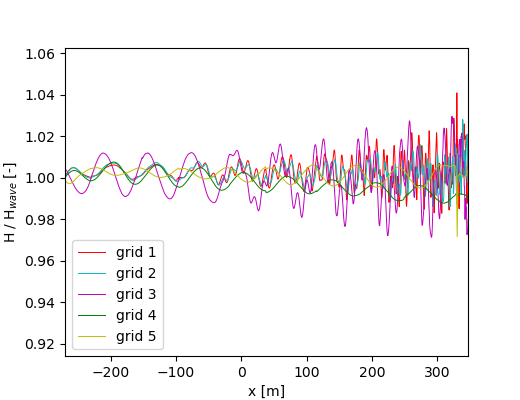
\includegraphics[width = \linewidth]{figures/Validation/numerical_dissipation.png}
%     \caption{Average wave height over length grid}
%     \label{fig:averagewaveheight}
% \end{figure}

What is interesting to note is that the coarse grids give good results in terms of reflection because they vary within 1\% of the incident wave height. There is a pattern of standing waves, which is the result of some of the wave energy reflecting off the outer boundary of the grid or at the refinement level edges. The finer grids, on the other hand, give oscillating results. The small y-axis limits are a bit misleading because the average wave height along the domain still varies within three per cent for the worst grid. 

% \textcolor{red}{It is not yet clear why the fine grids behave this way and a solution is currently being sought.} \\
The numerical dissipation that takes place over the length of the grid is better for fine grids. Especially in grid 5, the average wave height decreases in height as x increases, which means that the wave energy is lost through numerical dissipation as the wave propagates through the domain. 



\section{Wave interaction with a box-type breakwater}
\label{sec: box-type breakwater}
%box type
%Reflection
How ComFLOW deals with the reflection, transmission, and dissipation of wave energy when a box-shaped
structure interacts with regular waves is studied in this section. The comparison with the analytical formula for the transmission coefficient derived by \citet{macagno1953fluid} is made in Section \ref{subsec: Macagno formula}. The mean wave drift force acting on the structure is compared to the analytical mean wave drift force derived by \citep{longuethiggins1977}, in Section \ref{subsec: driftforces}. Both analytical formulas are derived by linear wave theory, so a long and shallow wave is simulated (H=0.5m and T=10.4s), to minimise the non-linear terms in the simulated waves. In this way a fair comparison can be made with the analytical formulas. \\
\\
For all grids, simulations are done with a box-type structure, with a varying width from 10 to 100 metres and a draught of 5 metres. It is placed in the grid in such a way that the right side of the box is always placed at x = 150 m. 

% -reflection is validated by the Macagno formula and the forces experienced.\\
% -explain relevance of Macagno formula and forces. Results compared with analytical values. A long and shallow wave (H=0.5 with T=10.4) is tested to reduce nonlinear effects.


\subsection{Macagno formula}
\label{subsec: Macagno formula}
The transmission coefficient $K_t$, which is the ratio between the transmitted wave height $H_t$ and the incident wave height $H_i$, is derived by \citet{macagno1953fluid} with linear wave theory.
% \begin{equation}
%     K_{\mathrm{t}}=\frac{1}{\sqrt{1+\left[\frac{k W_{\mathrm{f}} \sinh (k h)}{2 \cosh \left(k h-k T_{\mathrm{f}}\right)}\right]^{2}}}
%     \label{eq: macagno1953}
% \end{equation}


To compare these results to ComFLOW, the transmission coefficient $K_t = H_t / H_i$, the reflection coefficient $K_r = H_r / H_i$ and the dissipation coefficient $K_d$ are determined. The incident wave height $H_i$ is input (in this case: 0.5 metres), so only the transmitted wave height $H_t$ and the reflected wave height $H_r$ must be derived. The latter two can be used to quantify the loss/dissipation coefficient $K_d$.\\
\\
The \textbf{transmitted wave height $H_t$} is derived by averaging the mean wave height after the geometry. This is done in the same way as has been done for the wave-only cases discussed in Section \ref{sec: prop of free surface waves}, but now only between x = 190 m and x = 260 m. ComFLOW gives as output the water elevation over time for every cell in the x-direction at the waterline (which are 560 cells in total for grid 1). This averaging over 70 metres is convenient because this way the oscillating behaviour observed in Section \ref{sec: prop of free surface waves} is filtered (see Figure \ref{fig:averagewaveheight}). \\
\\
The \textbf{reflected wave height $H_r$} is determined via wave splitting theory according to \citet{Goda1976}, by comparing the time series of the water elevation between two points in front of the box, distancing a quarter of a wavelength from each other. This technique is explained extensively in Appendix \ref{app: wave splitting}.\\
\\
Now $H_i$,$H_t$ and $H_r$ are known, the \textbf{dissipation coefficient $K_d$} can be determined via the following derivation.
\begin{equation}
    H_t^2+H_r^2+H_d^2=H_i^2
\end{equation}
\begin{equation}
    K_d = \sqrt{1-K_t^2-K_r^2}
\end{equation}




\begin{figure}[h]
    \centering
    \begin{subfigure}[b]{0.49\textwidth}
        \centering
        \includegraphics[width=\textwidth]{figures/Validation/magagno_with_grid_simulations_eps.eps}
        \caption[]%
        {{\small Transmission, reflection and dissipation coefficient as function of floater width for all grids compared with the Macagno formula}}    
        \label{fig:Macagnocomparison}
    \end{subfigure}
    \hfill
    \begin{subfigure}[b]{0.49\textwidth}  
        \centering 
        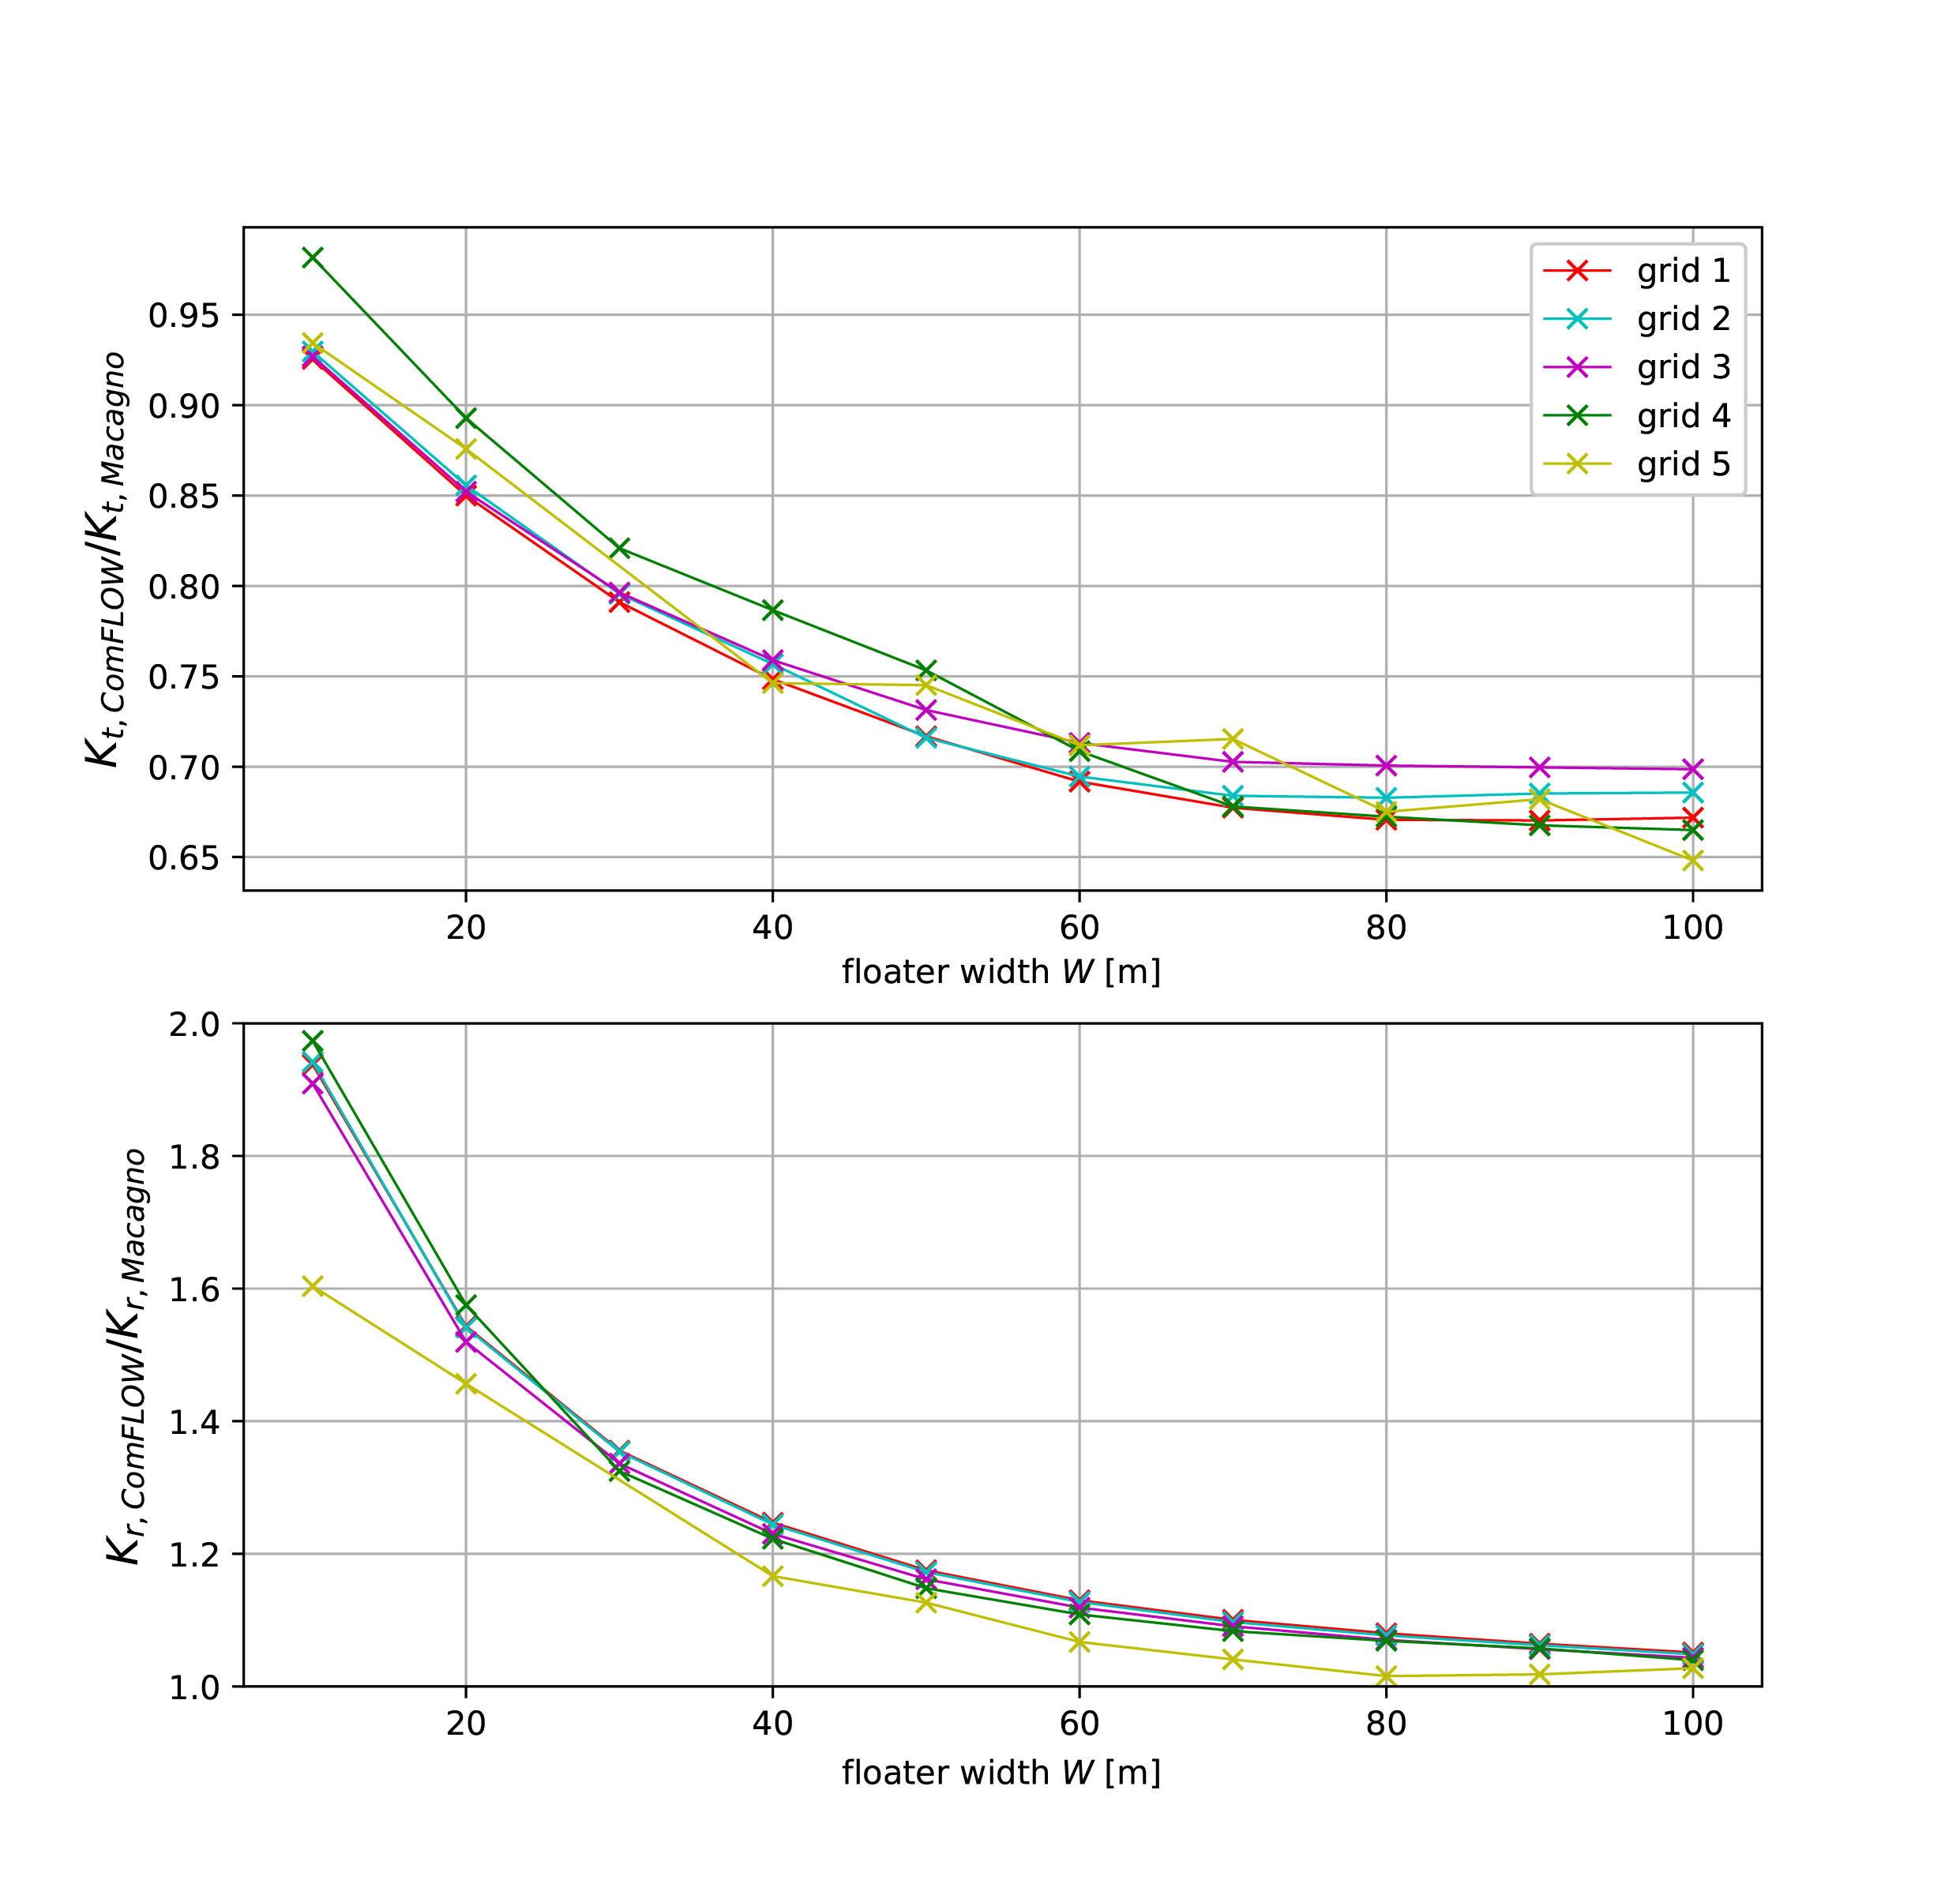
\includegraphics[width=\textwidth]{figures/Validation/magagno_offset_eps.png}
        \caption[]%
        {{\small Offset between ComFLOW results and linear wave theory}}    
        \label{fig:offset macagno}
    \end{subfigure}
    
    \caption{}
    \label{fig: }
\end{figure}

The results of ComFLOW, compared to the analytical Macagno formula, are plotted in Figure \ref{fig:Macagnocomparison}. 
The upper plot shows the transmission coefficient $K_t$. All grids, except grid 4, seem to converge to a static value in this plot. This static value follows the same trend as the analytical formula, but has an offset. Apparently, the transmitted wave height in ComFLOW is smaller than the transmitted wave height according to linear wave theory. What has been found is that if higher, steeper waves were simulated (i.e. nonlinearity increases), this difference in the analytical formula increases. So, this offset can be an indication that non-linearities are still present in the simulated waves. Also, this difference seems to get bigger while the box gets wider, which is an indication that nonlinearities are more dominant with a wider box.\\

The reflection coefficient $K_r$ is derived analytically from the Macagno formula (equation \ref{eq: macagno1953}) and $K_r^2 = 1 - K_t^2$. Here, the same effect is observed. The reflected wave height $H_r$ is observed to be larger in ComFLOW than according to linear wave theory, but this effect decreases as the box width increases. All grids except grid 5 seem to have converged to a static value in this plot.\\

% \begin{equation}
%     K_r = \sqrt{1 - K_t^2}
% \end{equation}


The lower plot shows the dissipation coefficient. Here, grids 4 and 5 give unrealistic results. Grids 1 and 2 have converged to a static value of around 0.1. This means that 10\% of the incoming wave height is dissipated by the presence of the box-type structure. Also, grid 3 is pretty close to convergence. \\
\\




In Figure \ref{fig:offset macagno} the offset is quantified. The upper plot shows that the difference in transmission coefficient $K_t$ between the ComFLOW results and the linear wave theory is 7\% for small widths and increases to 32\% for large box widths.
The reflection coefficient goes from 0.22 to 0.42, which is an increase of 91\% for the smallest box width simulated (W=10 m), but this increase increases to 4\% for the widest floaters. 
So, for short breakwaters, ComFLOW is more reflective, and for long breakwaters, ComFLOW is more dissipative than the Macagno formulation. 
% The results are plotted in Figure \ref{fig:Macagnocomparison}. With $K_t$ and $K_r$ as depending of the box width, grid 1 to 4 seem to converge to a constant solution, with an offset from the analytical formulas. The reflected wave height seems to be higher in the simulations and therefore, the transmitted wave height is lower as well. The lower plot shows the amount of dissipation as function of the width of the box. Grid 1 and 2 converged to each other from a box width greater than 50 meters. 

\subsection{Check other influences}

\subsubsection{Influence coarse grid near the bottom}
Since the coarse grid near the bottom covers a large part of the grid, a check is made to investigate whether its presence has any influence on the results. Therefore, four different floater widths \textit{W} are simulated and analysed. Figure \ref{fig:check coarse bottom} shows that the presence of the coarse grid near the bottom has no influence on the result of the transmission coefficient, so this is beneficial to keep it in future simulations.
% \begin{figure}[H]
%     \centering
%     \includegraphics[width=0.7\linewidth]{figures/Validation/magagno_investigation_fine_bottom.eps}
%     \caption{Investigation whether coarse bottom has a negative influence}
%     \label{fig:check coarse bottom}
% \end{figure}


% \subsubsection{Influence different ka}
% \begin{figure}[H]
%     \centering
%     \includegraphics[width=0.7\linewidth]{figures/Validation/magagno_investigation_different_kas.eps}
%     \caption{Influence of different wave steepnesses ka}
%     \label{fig:my_label}
% \end{figure}

\subsubsection{Influence different wave periods}
Different wave periods were also tested and compared to linear wave theory and resulted in similar percentage offsets. 
% \begin{figure}[H]
%     \centering
%     \includegraphics[width=0.7\linewidth]{figures/Validation/magagno_investigation_different_waveperiods.eps}
%     \caption{Different wave period compared to the Macagno formula}
%     \label{fig:different wave period check on macagno}
% \end{figure}



\begin{figure}[H]
    \centering
    \begin{subfigure}[b]{0.49\textwidth}
        \centering
        \includegraphics[width=\textwidth]{figures/Validation/magagno_investigation_fine_bottom.eps}
        \caption[]%
        {{\small}Investigation whether a coarse grid near the bottom has a negative influence}    
        \label{fig:check coarse bottom}
    \end{subfigure}
    \hfill
    \begin{subfigure}[b]{0.49\textwidth}  
        \centering 
        \includegraphics[width=\textwidth]{figures/Validation/magagno_investigation_different_waveperiods.eps}
        \caption[]%
        {{\small}Different wave period compared to the Macagno formula}    
        \label{fig:check different periods macagno}
    \end{subfigure}

    
    \caption{}
    \label{}
\end{figure}



\subsection{Drift forces}
\label{subsec: driftforces}
The forces in ComFLOW are determined by integrating the pressure over the surface of the geometry. The first-order wave forces have the same frequency as the wave frequency. The raw output from ComFLOW is subject to high-frequency oscillations due to the rapid pressure fluctuations around the structure. Therefore, all frequencies above twice the wave frequency are filtered out of the signal, resulting in the time series of the total wave force where the first-order component is clearly visible (see Figure \ref{fig:forceovertime}).\\
\begin{figure}[H]
    \centering
    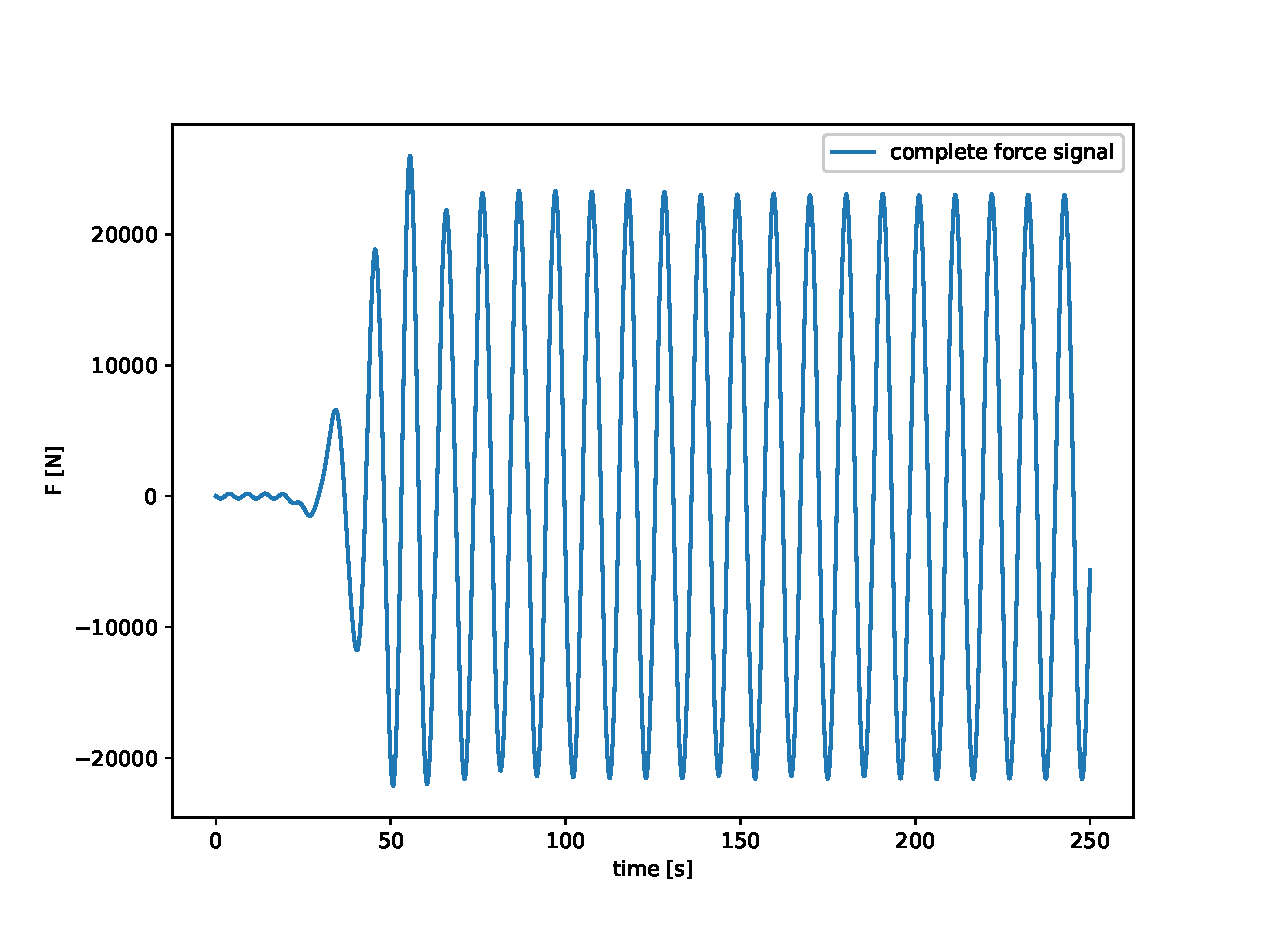
\includegraphics[width=0.6\linewidth]{figures/Validation/forcesignal_on_single_box_eps.eps}
    \caption{Force in x-direction on the box over time}
    \label{fig:forceovertime}
\end{figure}
The filtered signal (in Figure \ref{fig:forceovertime}) was needed by automatically determining when the waves were fully developed and for cutting part of the simulation to reach an integer amount of waves. However, the unfiltered output of ComFLOW is used in the calculation of the mean wave drift force. This is done for different widths of the box, for all grids studied, resulting in a mean wave drift force for each configuration and is compared to the analytical value of the mean wave drift force according to \citet{longuethiggins1977} in Figure \ref{fig:meanforceanalyticalcomparison all grids}. From which it is easily observable, grid 3 t/m 5 gives very unrealistic results. Therefore, they are discarded in Figure \ref{fig:meanforceanalyticalcomparison two grids}.

% \begin{figure}[H]
%     \centering
%     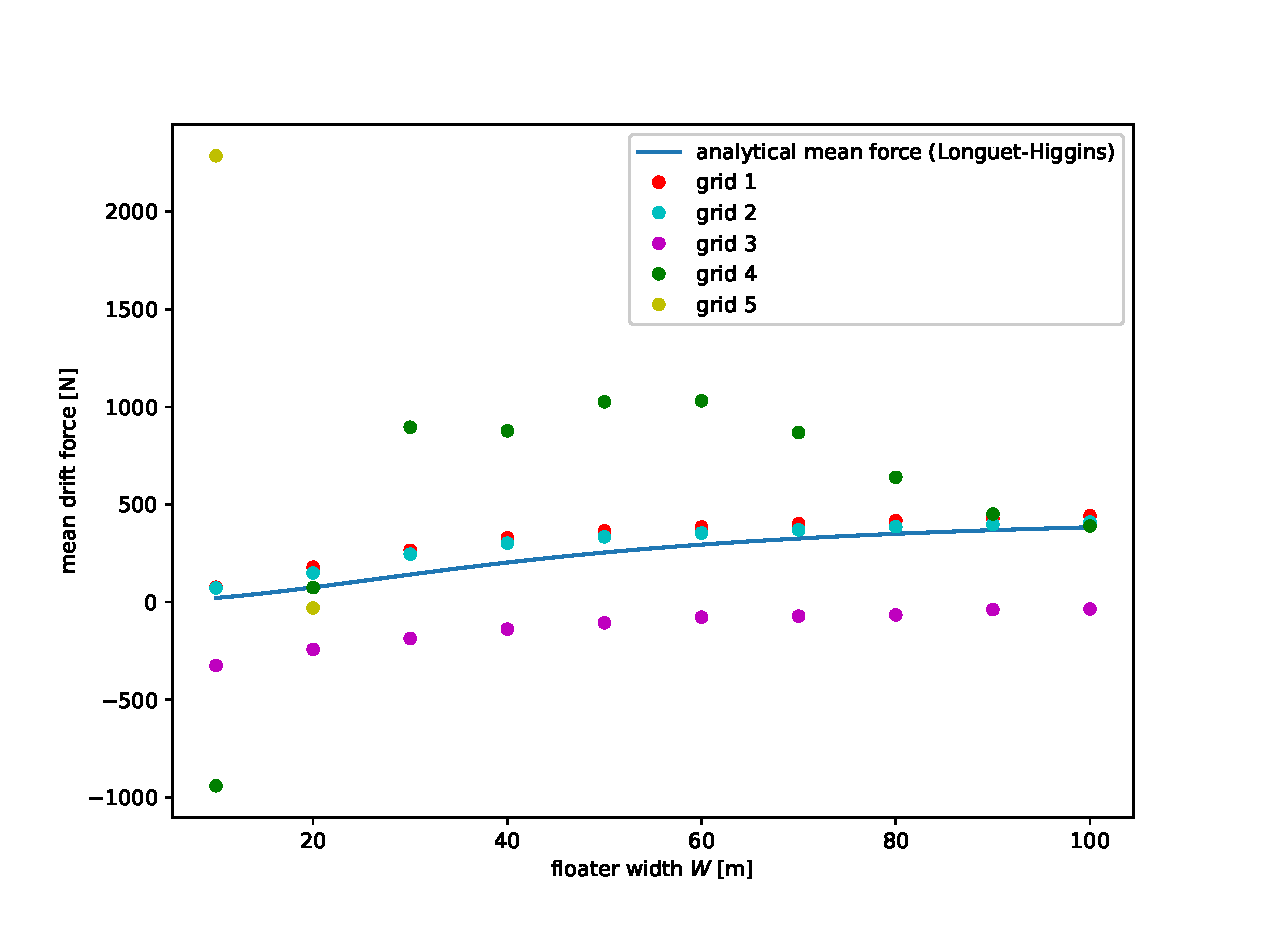
\includegraphics[width=\linewidth]{figures/Validation/forces_with_all_grids.eps}
%     \caption{Mean force on box in x-direction as function of width of the box, all grids}
%     \label{fig:meanforceanalyticalcomparison all grids}
% \end{figure}

In Figure \ref{fig:meanforceanalyticalcomparison two grids} both grids with applicable results (grids 1 \& 2) are shown. As can be seen in Table \ref{tab:celldimensions}, grid 1 took four days to compute, which is disproportionately high for this kind of simulation. Therefore, the results of grid 1 are considered the best ComFLOW can get and are used as a benchmark to determine the optimal grid. Grid 2 converged to this solution, with a small offset. The solid line is the analytical force, where the reflected and transmitted wave height is calculated with the Macagno formula \ref{eq: macagno1953} \citep{macagno1953fluid} and the force is calculated with equation \ref{eq: longuethiggins force}, derived by \citet{longuethiggins1977}. The dashed lines are also calculated with equation \ref{eq: longuethiggins force}, but with the wave heights determined by the output of the ComFLOW simulations. These dashed lines comply with the force output of ComFLOW, which means that the calculation of the force acting on the structure is very accurate, but the determination of the reflected and transmitted wave height is a bit off. This is an interesting and useful result, as the actual wave height in ComFLOW can be easily determined. Therefore, a qualitative analysis can be done for the drift forces on the structure. In the previous section, the reflected wave height was found to be higher in ComFLOW than according to the linear wave theory (see Figure \ref{fig:Macagnocomparison}). More reflection on the structure results in a higher mean wave drift force (according to equation \ref{eq: longuethiggins force}). Therefore, the greater force found by ComFLOW compared to linear wave theory was expected since the analysis of Section \ref{sec: box-type breakwater}.


% %difference in results are clearly not from the calculation of the forces, but from the numerical dissipation? not sure though?
% \begin{equation}
% F=\frac{1}{4} \rho g\left(a_i^{2}+a_r^{2}-a_t^{2}\right)(1+ \frac{2 k h}{\sinh 2 k h})
% \label{eq: force longuet}
% \end{equation}

% \begin{figure}[H]
%     \centering
%     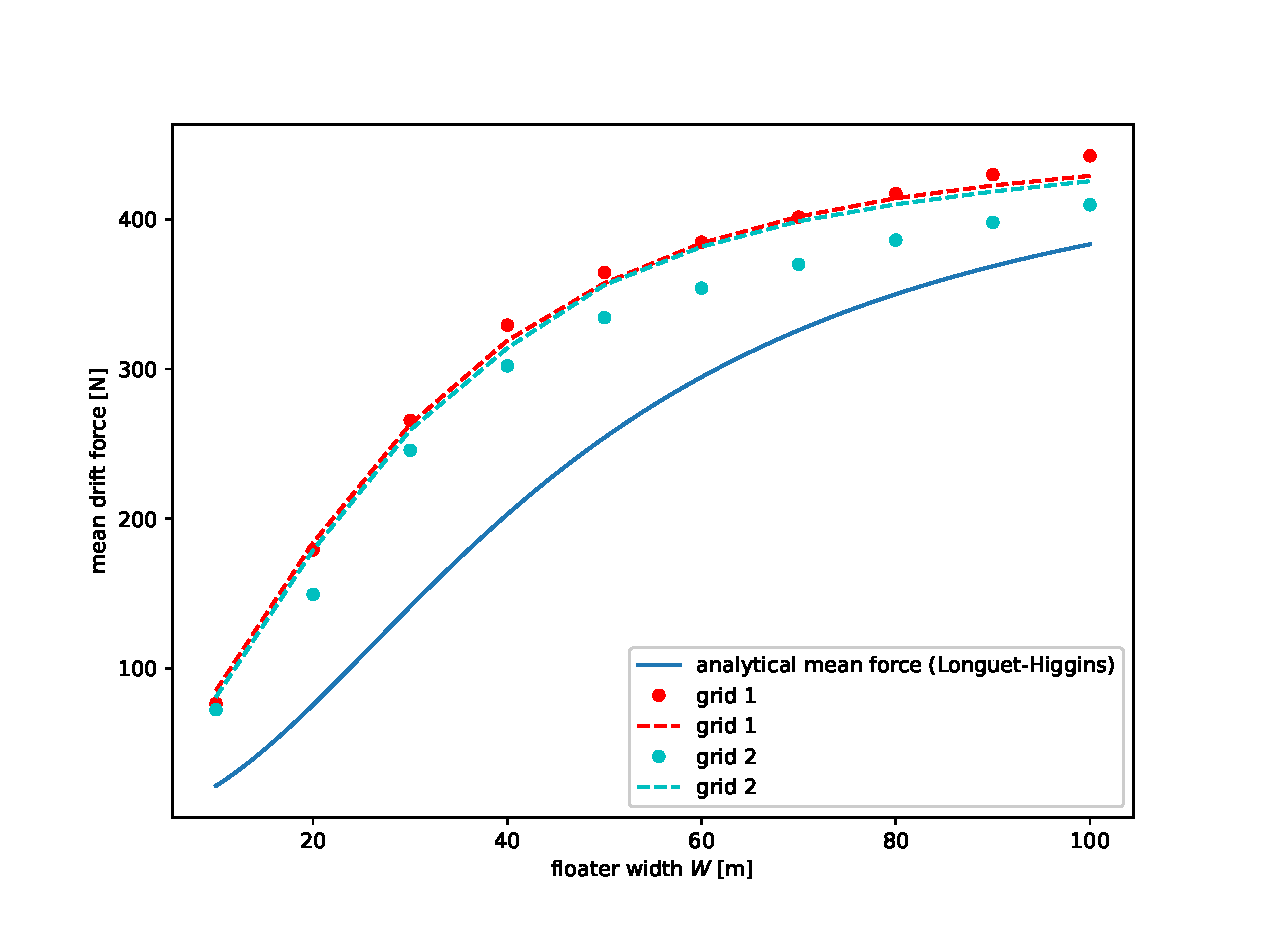
\includegraphics[width=\linewidth]{figures/Validation/forces_with_two_grids_inc_semi_analytical_eps.eps}
%     \caption{Mean force on box in x-direction as function of width of the box, two finest grids}
%     \label{fig:meanforceanalyticalcomparison two grids}
% \end{figure}

\begin{figure}[H]
    \centering
    \hfill
    \begin{subfigure}[b]{0.49\textwidth}  
        \centering 
        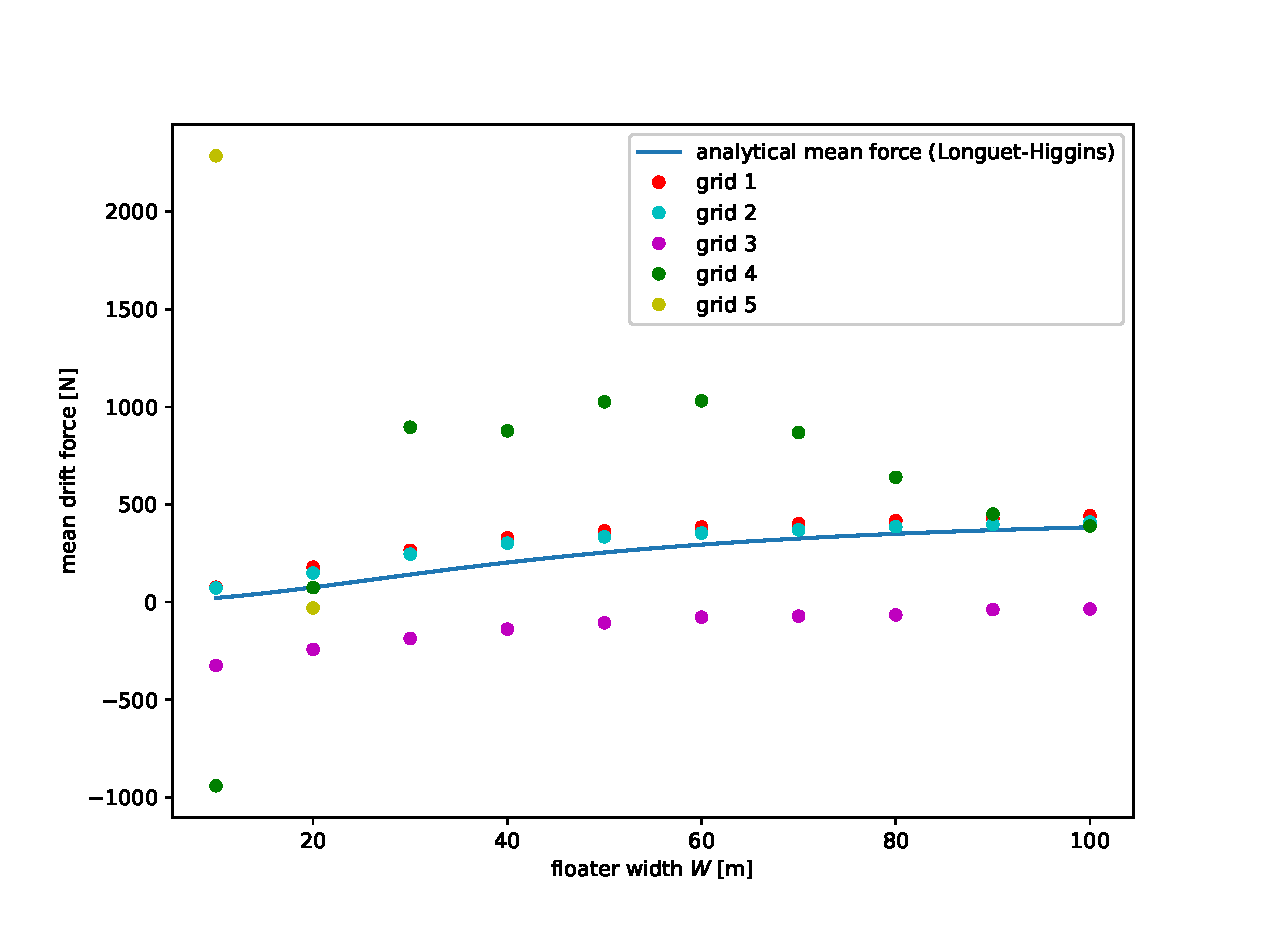
\includegraphics[width=\textwidth]{figures/Validation/forces_with_all_grids.eps}
          \caption[]%
        {{\small}Mean force on box in x-direction as function of width of the box, all grids} 
        \label{fig:meanforceanalyticalcomparison all grids}
    \end{subfigure}
    \hfill
    \begin{subfigure}[b]{0.49\textwidth}
        \centering
        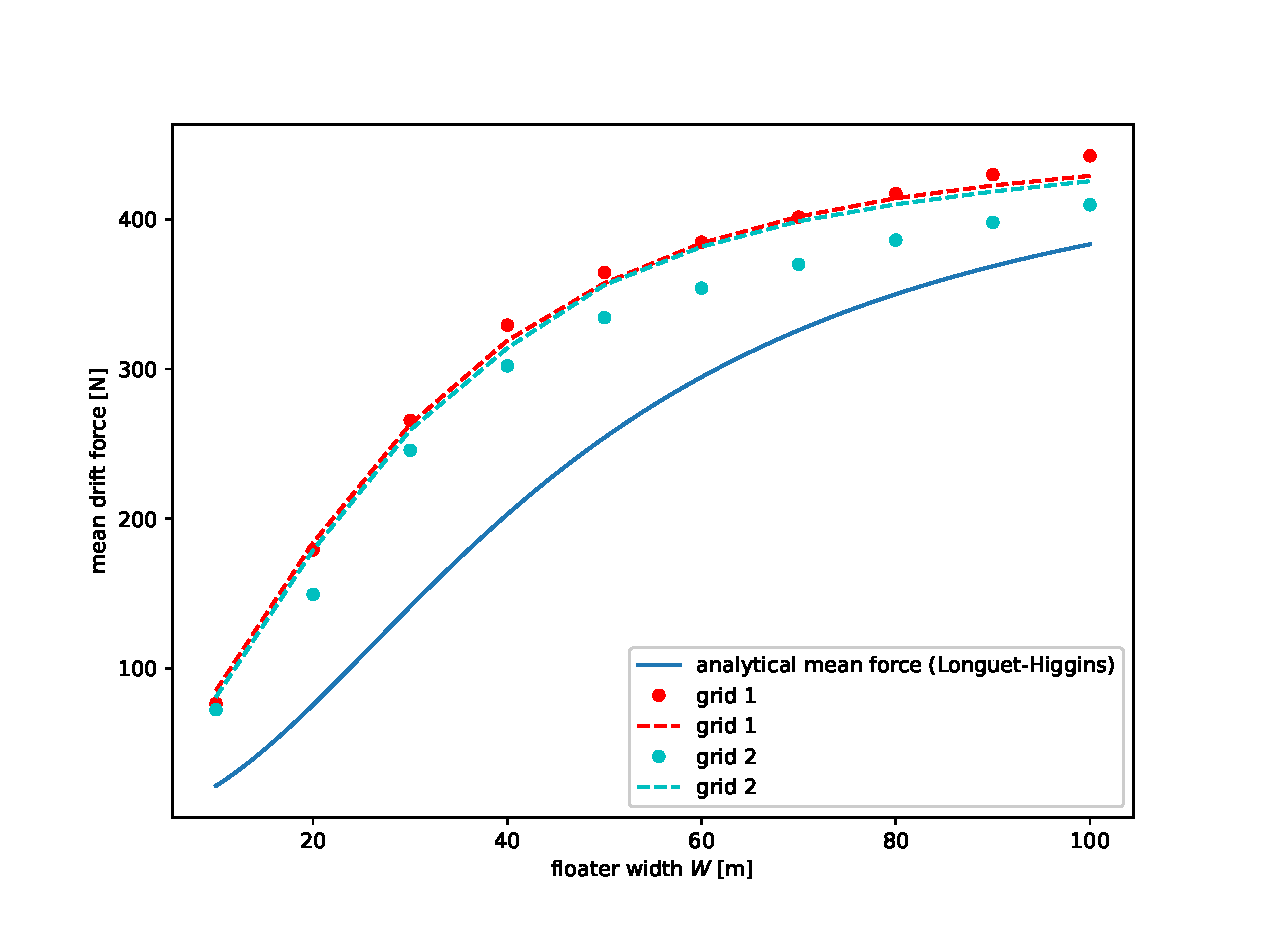
\includegraphics[width=\textwidth]{figures/Validation/forces_with_two_grids_inc_semi_analytical_eps.eps}
        \caption[]%
        {{\small}Mean force on box in x-direction as function of width of the box, two finest grids}    
        \label{fig:meanforceanalyticalcomparison two grids}
    \end{subfigure}
    
    \caption{}
    \label{}
\end{figure}


\section{Energy dissipation through wave breaking}
\label{sec: Dissipation}
%breaker bar
%-An experiment with a breaker bar is mimicked to validate the model on dissipation


As explained in detail in Section \ref{subsec: comflow literature review}, the physical dissipation characteristics in ComFLOW are expected to depend strongly on the grid size in the area where the waves will break. To map this effect, a validation is performed where an experiment, done by  \citet{breakerbarexperiment}, where waves were plunging over a breaker bar, is mimicked in ComFLOW, after which both results were compared. Furthermore, the results of this validation are used to design the correct grid for future simulations by verifying what combination of incident wave height and grid size results in reasonable dissipation rates when waves break.

\subsection{Experiment breaker bar}
A large-scale wave flume experiment has been carried by \citet{breakerbarexperiment} out involving a T = 4s regular wave with H = 0.78 m wave height plunging over a fixed barred beach profile. In the top plot of Figure \ref{fig:breakerbarexperiment}, the bathymetry of the experiment is shown. The waves were generated by a wave paddle at x = 0 and propagated to the right. Elevations of the surface of the water were measured with resistive wave gauges mounted on the side wall at 19 locations along the flume, from x=12 m in the constant depth section of the flume to x=49 m in the shoaling zone. Resistive wave gauges were not deployed in the surf zone since they suffered from spurious measurements due to the strong splash-up of water. For the remainder of the profile, pressure transducers (STS-ATM/N) were therefore fitted along the flume sidewall at an approximate 0.5 m spacing. The elevations of the water surface were retrieved from the pressure measurements after correction for pressure attenuation due to depth using linear wave theory. \\
\\


\subsection{Grid settings}

This experiment has been simulated in ComFLOW, with a uniform grid over the entire domain. The purpose is to give an insight into what settings to use and how fine the grid needs to be around the geometry later on in this project, where wave breaking will occur as well. The exact dimensions of the cell sizes of the different grids are shown in the legend from Figure \ref{fig:breakerbarexperiment}. 



% -to find the optimal grid refinement for around the geometry where the dissipation occurs, an experiment is compared with ComFLOW results.
%  -show the effect of breaking on convection scheme (refer to paragraph: convection scheme, in section settings)
% -standing wave pattern as expected, difficult to measure wave height when breaking (liquid fill ratios are used, so when lots of air in wave, unrealistic values), doesn't matter, as long as $a_i$ and $a_t$ are corresponding and they do.
% %- put some statistics in here, thrustworthy interval, some boxplots on how much the ComFLOW simulations could be trusted

\begin{figure}[H]
    \centering
    \includegraphics[width=0.8\linewidth]{figures/Validation/plot_stats_compare_H-1.eps}
    \caption{Results different grids in ComFLOW with experiment \citep{breakerbarexperiment}}
    \label{fig:breakerbarexperiment}
\end{figure}


The results show that the wave height behind the breaker bar (58m < x < 63 m) corresponds very well to the experiment for all grids except the one indicated with the orange line in Figure \ref{fig:breakerbarexperiment}. The wave height in front of the breaker bar (x < 50 m) corresponds to the experiment for all grids except the one with cell dimensions with dx and dz of 500 mm. What is interesting to note is that the mean water level (third plot in Figure \ref{fig:breakerbarexperiment}) is generally higher than in the experiment.  Also, ComFLOW does not seem to take the set-down when waves get very steep before breaking into account. \\
The wave height exactly at the breaking point (x = 53m) does not correspond at all to the experiment, and the different grids differ here as well. This is because much air is intruded into the water at the moment of breaking. ComFLOW determines the elevation of water by checking the liquid fill ratios of each cell and adding the amount of water in a vertical column of cells. Therefore, when lots of air is intruded into the water, ComFLOWs results might differ from the actual height of the waves. In addition, measurements of the wave height of a wave with a lot of entrapped air in the experiments are not trivial as well. In other words, the measurements of the experiment at position 50 m < x < 54 m are also not inviolable. For further simulations, this is no problem at all, since only the transmitted wave height, reflected wave height, and incident wave height need to be determined in order to derive the amount of wave energy lost in the breaking process. The difference in wave height between the different grids can also be declared by the difference in numerical dissipation. The green line (with a dx and dz of 500 mm) dissipates the most during shoaling, which is quite logical because this grid is very coarse. \\


\subsection{Convection scheme}
\label{subsec: breakerbar on convection scheme} 
The convection scheme seems to have a significant impact on the breaking characteristic of ComFLOW, which can be seen in Figure \ref{fig:breakerbarexperiment convection scheme}. Here, both convection schemes (first-order upwind and second-order central) have been simulated with the same grid, with cell size: dx = 50mm and dz = 25mm. The second-order central convection scheme gave less favourable results than the first-order upwind scheme. The wave height after the breaker bar differs more from the experiment's measurements (see Figure below). Furthermore, the second-order central convection scheme resulted in very high local fluid velocities in the breaking process. Thus, the time step per computation will be high, which results in unreasonably large execution times.\\
\\
This poor behaviour of the second-order central method might be due to the fact that this method uses three cells in order to do one discretization (see SubSection \textbf{Convection scheme} of Section \ref{subsec: numercial settings validation}), while the first-order upwind method uses two cells. Since the breaking process takes place around the water line and tiny air pockets get entrained in the water as well during breaking, the discretization must deal with these two mediums in the flow at a low-dimensional scale. Therefore, it might be too much to accurately do a discretization using three cells. So, although second-order discretizations tend to be more accurate in general, because they take into account second-order terms, this is not the case for the simulation of breaking waves. 



\begin{figure}[H]
    \centering
    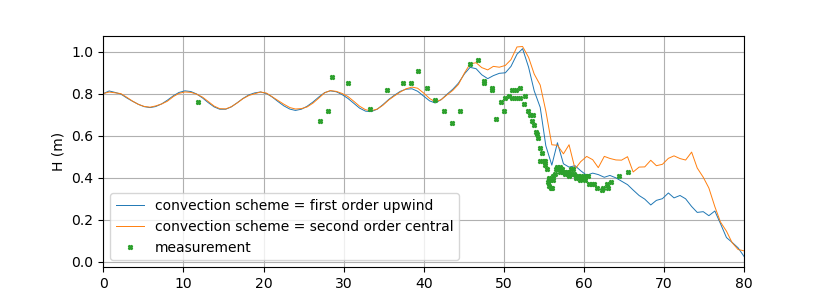
\includegraphics[width=\linewidth]{figures/Validation/plot_stats_compare_H-1_2ndordercentral.png}
    \caption{Influence of convection scheme on breaking characteristics}
    \label{fig:breakerbarexperiment convection scheme}
\end{figure}


% \section{Final settings used in ComFLOW}
% The settings which were found to be best performing are:
% \begin{itemize}
%     \item 
% \end{itemize}

% As mentioned before, the grid dimensions should scale to the properties of the wave. The research in this validation is done with a regular wave with H = 0.5m and T = 10.4s. To make sure the results are applicable to future waves, the cell dimensions of the best performing grid is non-dimensionalized w.r.t. the wave dimensions in the following Table:






%three different HKN waves


\section{Discussion}
The results of ComFLOW were analysed and compared to analytical formulas, and an experiment to make sure its results are reliable and give a good representation of reality. Therefore, the analytical formula for the transmission coefficient: the Macagno formula, derived by \citep{macagno1953fluid}, and the analytical formula for the mean wave drift force, derived by \citep{longuethiggins1977}, are compared with the results of ComFLOW by simulating a regular wave of H=0.5 m, T=10.4 s in a water depth of 23 metres for 250 seconds. Furthermore, a fast, but reliable simulation is desired, and therefore the propagation of free surface waves was studied to map the computation time and the numerical dissipation throughout the grid. This also contributes to choosing the right grid for the simulations. Lastly, an experiment where waves were breaking over a breaker bar was mimicked in ComFLOW to compare the experimental outcome with ComFLOWs results. Therefore, the dissipation characteristics of ComFLOW are mapped.
\\
Five different grids were tested, numbered from grid 1 to 5 sorted according to refinement, where grid 1 was the finest and grid 5 the coarsest. Grid 1 took more than four days to compute with its 5 million cells. Grid 2, containing roughly one and a half million cells, converged to the same solutions as grid 1 but took only 13 hours to compute. Grid 3, 4 and 5 gave unreliable results; where the forces resulting from the simulations with these grids were either extremely high or extremely low, sometimes even negative. So, the coarseness of grid 2 is labelled as best for the simulation with a regular wave with characteristics: H=0.5 m and T=10.4 s. Therefore, since grid 2 has a cell height and width of 250 mm and the draught of the box-type breakwater is five metres, 20 cells are necessary over the height of the geometry to give reliable forces in the x-direction. Although the grid refinements used lead to a converged result (i.e., independently of further refinements) which follows the same trend as the analytical formulas, it still gives an offset to the analytical formulas corresponding with linear wave theory. The transmitted wave height measured in the simulations with ComFLOW was too low, and the reflected wave heights were too high. The mean wave drift forces were also a bit too high, which is due to the excessively high reflection coefficient. \\
The comparison with ComFLOW and the experiment in which waves plunged over a breaker bar showed good results. The height of the wave behind the breaker bar matched well for all grids on the grid with dx=200mm and dz=200mm. In other words, the dissipation of wave energy by breaking was well simulated in ComFLOW. The height of the wave at the breaking point and the mean water level did not match the measurements of the experiment.

% %The fist sub-research question can be answered already: what is the quality of ComFLOW and untill what extend can it be used compared to real life situations?
% \textbf{This dashed lines comply with the force output of ComFLOW, which means the calculation of the force acting on the structure is very accurate, but the determination of the reflected and transmitted wave height is a bit off. This is an interesting and usefull result, since the actual wave height in ComFLOW can be determined easily. Therefore, a qualitative analysis can be done for the drift forces on the structure. }


% feedback Peter:
% \textcolor{red}{\textbf{it is not the best possible grid, but the best possible grid that I can buy}}


% %in hoeverre kan je vertrouwen op de ComFLOW dissipatie validatie?
% -shortages of ComFLOW (viscous effects too strong)

% -shortages of regular waves:\\
% Since the continuous contribution of different frequencies in a irregular wave spectrum, the natural period of a floating system will often comply with one of the wave frequencies. This will lead to large excitations (see Figure \ref{fig:largeexcitation_lowfreq} from \citep{journee2000offshore}) and mooring system forces will be dominated by this effect; its design must account for this. 
% But, with regular waves, it is highly likely this phenomena will not occur.....

%  "Later, higher waves in which the higher harmonics are more dominant can be tested and compared with the results of this section in order to quantify the magnitude of the nonlinear terms of the waves.", from Section \ref{subsec: Macagno formula}. This magnitude is not validated, so this guarantees not it is the same.

% -dissipation depends on fineness grid..
\section{Conclusions}

So the coarseness of grid 2 is labelled as best for the simulation with a regular wave with characteristics: H=0.5 m and T=10.4 s. Therefore, since grid 2 has a cell height and width of 250 mm and the draught of the box-type breakwater is five meters, twenty cells are necessary over the height of the geometry to give reliable forces in the x-direction. \\
\\
ComFLOW's results for the transmission coefficient with a varying box width follow the same trend as expected by the Macagno formula, which is a function derived from linear wave theory. Wave transmission is lower in ComFLOW than in linear wave theory: 7\% for small box widths (W=10 m) and increases to 32\% for large widths (W=100m). Wave reflection is higher: 91\% for the smallest box width and 4\% for the widest floaters. \\
\\
All different grid sizes used in the comparison with the experiment were waves plunged over a breaker bar showed results that were in compliance with the experiment. 